\documentclass[tikz,border=10pt]{standalone}
\begin{document}
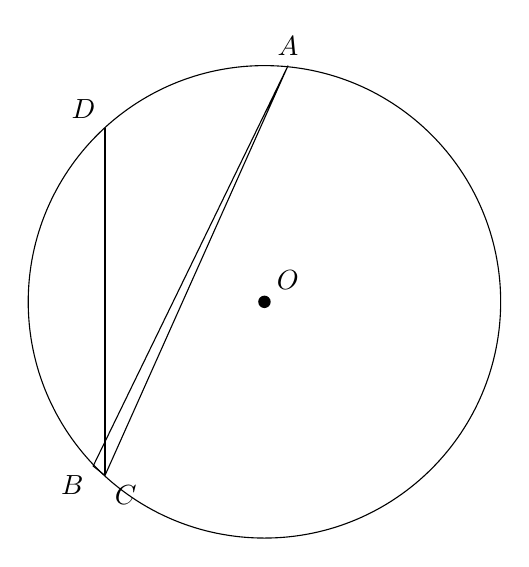
\begin{tikzpicture}[scale=1.5]
  \coordinate (O) at (0,0);
  \coordinate (A) at (0.2,2);
  \coordinate (D) at (-1.35,1.47);
  \coordinate (C) at (-1.35,-1.47);
  \coordinate (B) at (-1.45,-1.39);
  \draw (O) circle (2);
  \draw (A) -- (B) -- (C) -- cycle;
  \draw (D) -- (C);
  \fill (O) circle (1.5pt);
  \node[above] at (A) {$A$};
  \node[above left] at (D) {$D$};
  \node[below left] at (B) {$B$};
  \node[below right] at (C) {$C$};
  \node[above right=1pt] at (O) {$O$};
\end{tikzpicture}
\end{document}
